\documentclass{article}
\usepackage[utf8]{inputenc}
\usepackage{amsmath}
\usepackage{amssymb}
\usepackage{amsfonts}
\usepackage{amssymb}
\usepackage{minted}
\usepackage{graphicx}
\graphicspath{ {img/} }
\usepackage{titlesec}
\usepackage[a4paper,margin=1in,footskip=0.25in]{geometry}
\usepackage{fancyhdr}
\pagestyle{fancy}
%basic page layout

%draw finite state machine
\usepackage{tikz}
\usetikzlibrary{arrows,automata}
\newcommand{\hwnumber}{2}
\newcommand{\Lcvy}{\mathcal{L}}
%header and footer settings
\lhead{Algorithms and Data Structure \hwnumber}
\chead{Yiping Deng}
\rhead{\today}

\titlelabel{\thetitle\enspace}

\begin{document}
\title{Algorithms and Data Structure \hwnumber}
\author{Yiping Deng}
\maketitle
\thispagestyle{fancy}
\section*{Problem 1}
\subsection*{(a)}
The concrete implementation is here:
FILE 1: MergeSortVariant.scala
\inputminted{Scala}{MergeSortVariant/src/main/scala/MergeSortVariant.scala}
FILE 2: Timer.scala
\inputminted{Scala}{MergeSortVariant/src/main/scala/Timer.scala}
\subsection*{(b)}
The Scala main function will generate the data necessary for plotting.
Plotting is performed by Python.
\inputminted{Python}{plot.py}
\textbf{red} line denotes worst case, \textbf{green} line denotes average case, \textbf{blue} line denotes best case.
x-axis denotes k, y-axis denotes running time. \\
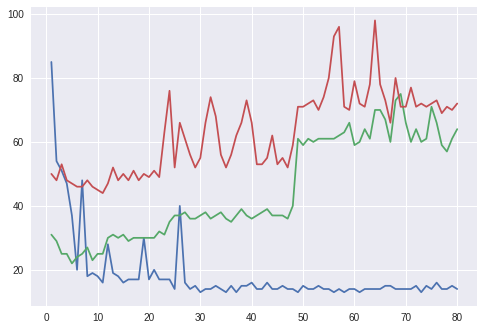
\includegraphics{plot.png}
Also the graph along with input size n with k = 20 \\
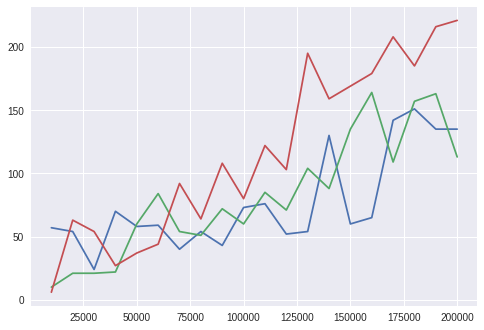
\includegraphics{k20.png}
The graph alogn with input size n with k = 50 \\
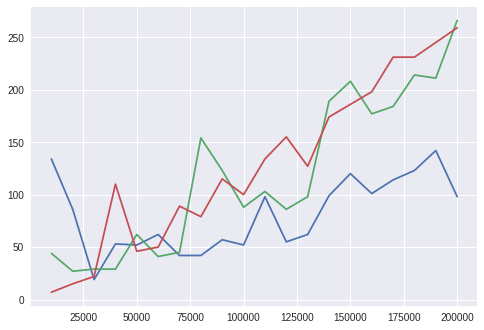
\includegraphics{k50.png}

\subsection*{(c)}
As you can see in picture 1, the best case running time is decreasing when k is increasing.
Worst case running time is increasing as k increased.
Average case reach its minimum when k is around 5
\subsection*{(d)}
We can use the graph, in the first picture, find the minimum of running time with respect to k.
Make sure the input size is big enough and it is random to represent averge case.

\section*{Problem 2}
\subsection*{(a)}
$ a = 36$, $b = 6$, $f(n) = 2n \implies$ $f(n) \in O(n^{log_b a}) \implies T(n) = \Theta(n^2) $
\subsection*{(b)}
$ a = 5$, $b = 3$, $f(n) = 17n^{1.2} \implies f(n) \in O(n^{log_b a} \implies T(n) = \Theta(n^{log_3 5)}$
\subsection*{(c)}
$ a = 12$, $b = 2$, $f(n) = n^2 lg(n) \implies f(n) \in O(n^{log_b a} \implies T(n) = \Theta(n^{log_2 12})$
\subsection*{(d)}
Using the tree method and draw the tree, we have

In this result, the first term, $2^n$, dominates the rest of term in the summation of the tree$ (2^{1/2})^n $ , $ (2^{1/5})^n ...$. 
Thus, the result is $ \Theta(n^2) $ \\
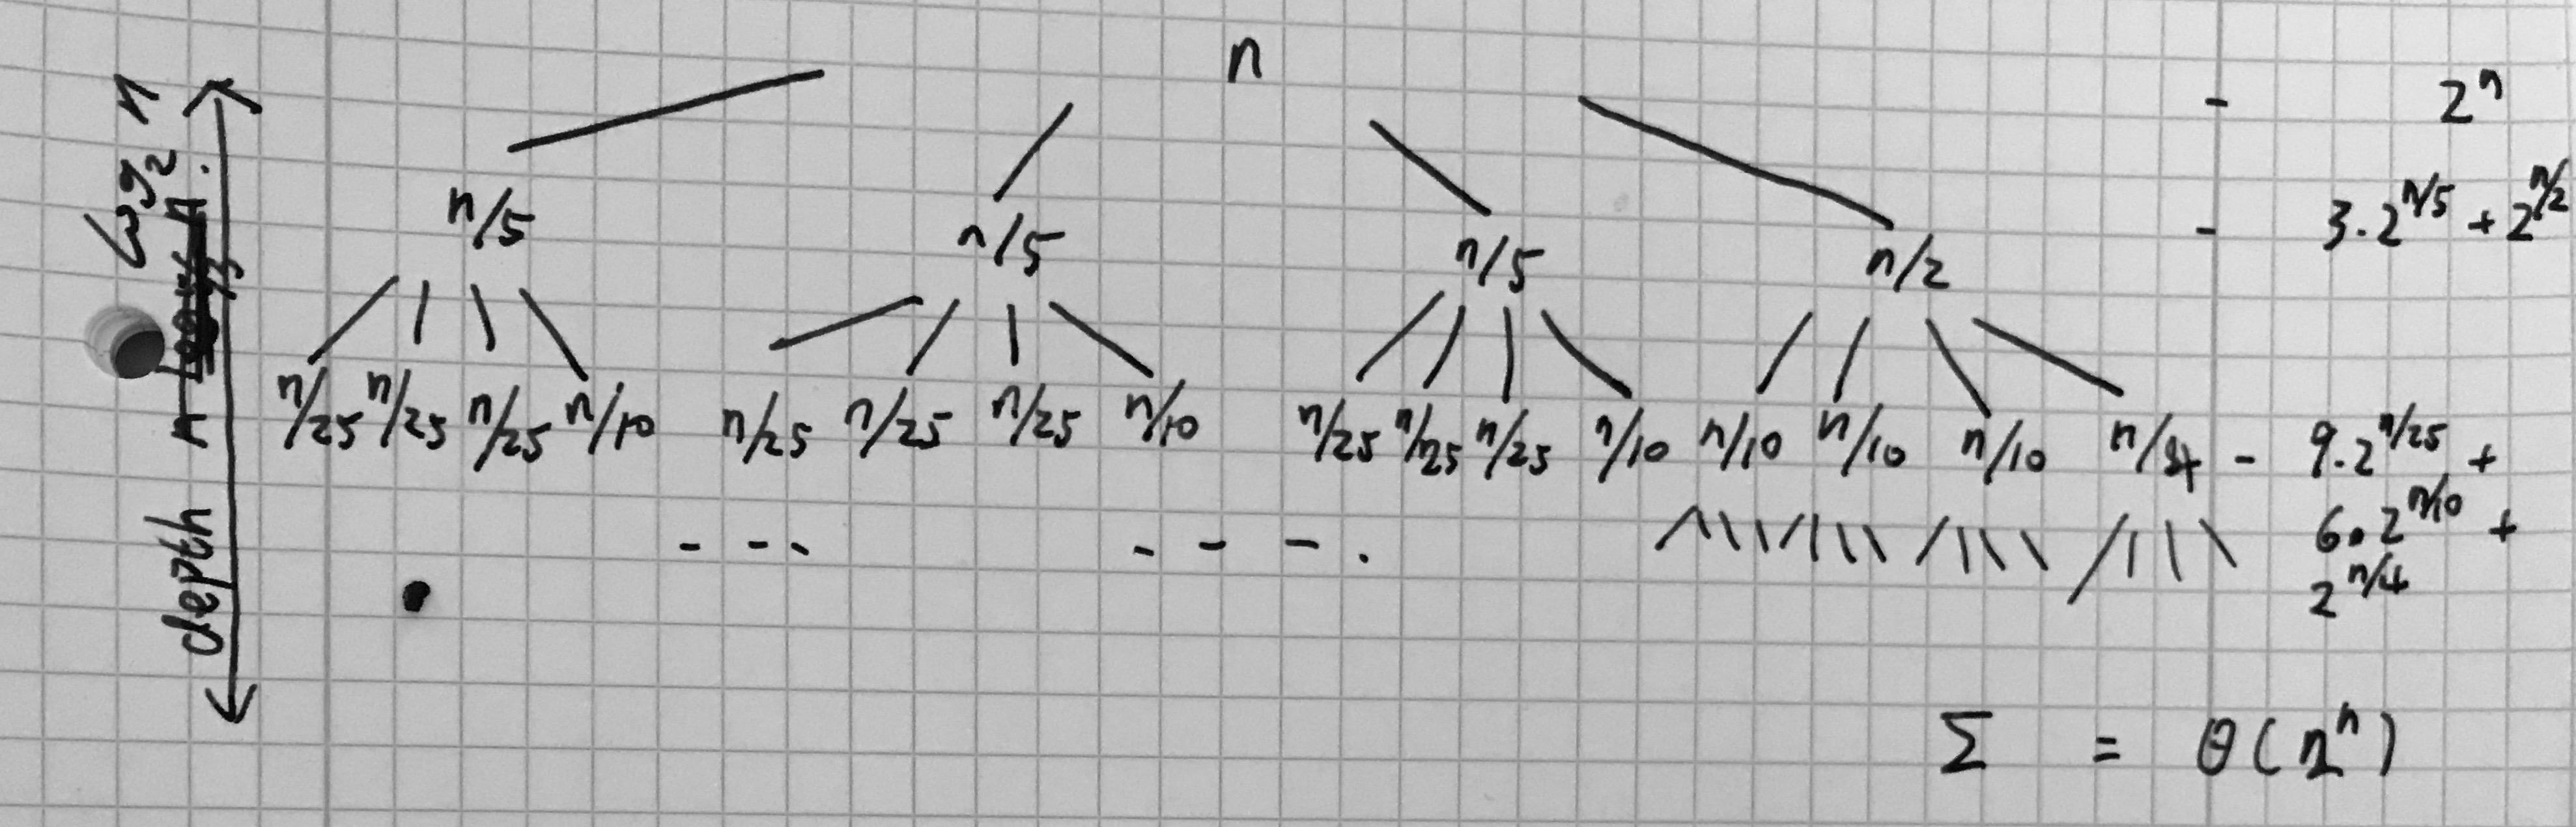
\includegraphics[width=\textwidth,height=\textheight,keepaspectratio]{tree1.jpg}
\subsection*{(e)}
Again, from tree method, the height of the tree is $log_{5/3} n$ at most, $log_{5/3} n$ at least. At each level of trees, there are n operations.
Thus, we can safely conclude that it is $\Theta(n \log n)$ \\
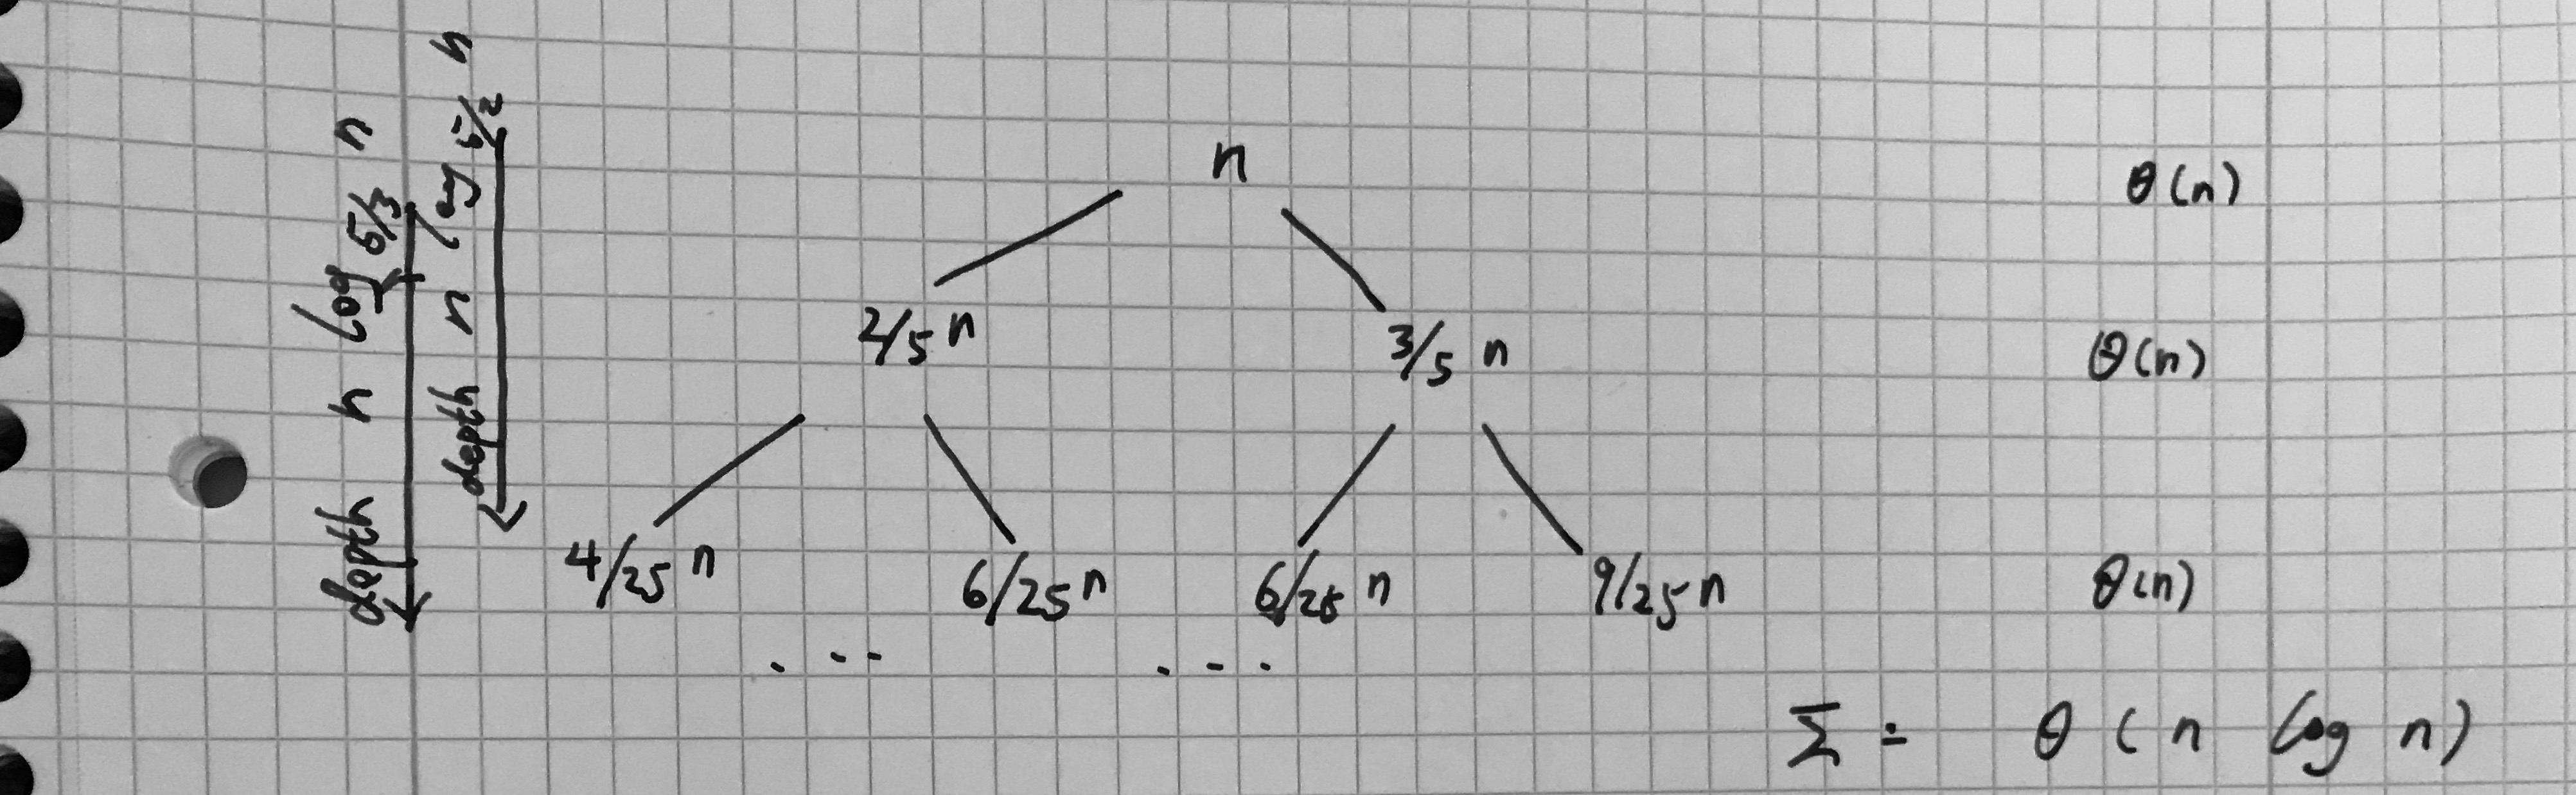
\includegraphics[width=\textwidth,height=\textheight,keepaspectratio]{tree2.jpg}
\end{document}
